\documentclass[10pt,letterpaper]{article}
\usepackage[margin=1in]{geometry}
\usepackage[OT1]{fontenc}
\renewcommand{\rmdefault}{ptm}
\usepackage{amsmath,amssymb,graphicx,booktabs,array,float}
\usepackage[font=small,labelfont=bf]{caption}
\usepackage{microtype}
\usepackage{xcolor}
\usepackage[hidelinks]{hyperref}
\usepackage{url}
\definecolor{navy}{HTML}{16324F}
\newcommand{\unit}{\ensuremath{\mathrm{m\,s^{-2}}}}
\newcommand{\R}{\mathbb{R}}
\setlength{\parindent}{1em}
\setlength{\parskip}{2pt}
\setlength{\textfloatsep}{9pt}
\setlength{\intextsep}{8pt}
\renewcommand{\arraystretch}{1.12}
\urlstyle{same}
\hypersetup{pdftitle={Learning Corrections to Drone Motion Models},pdfauthor={Emilio Sebastian Daza Vigo}}
\begin{document}
\begin{center}
{\LARGE\bfseries Learning Corrections to Drone Motion Models}\par
\vspace{5pt}
{\large Emilio Sebastian Daza Vigo}\par
CS 74 Final Project \quad Track 3 \quad November 13, 2026
\end{center}
\vspace{-8pt}
\begin{abstract}
This project tests whether a small neural residual improves a simplified quadrotor thrust model and whether its benefit changes with flight speed. Five regressors predict the released NeuroBEM body-frame acceleration channels from ten contemporaneous inputs. All segments of each flight remain in one partition, with 65 training, 17 validation, and 13 test flights. Across three training seeds, direct and residual networks attain overall test RMSEs of $0.4985$ and $0.4906$~\unit, respectively. Below $5$~m/s, the direct network performs better. At or above $5$~m/s, the residual network reduces pooled RMSE by $2.7\%$ and outperforms the direct network on 10 of 12 eligible flights. A separate Isaac Sim showcase does not preserve this ranking: the direct controller tracks slightly better at an initial speed of $6$~m/s. The results support a modest, speed-dependent prediction benefit within this dataset, with limited evidence for improved control.
\end{abstract}
\vspace{-9pt}
\section{Problem, motivation, and related work}
Simple rotor-thrust approximations make drone dynamics interpretable and inexpensive to evaluate, but omit velocity-dependent aerodynamic effects. Learning their remaining errors offers a possible compromise between a fixed physical approximation and a fully learned predictor. The research question is: \emph{At which flight speeds does learning a correction improve acceleration prediction on unseen flights, and when do linear regression or direct neural prediction perform as well?} The hypothesis is that omitted aerodynamic effects make a learned correction more useful at higher speeds.

NeuroBEM combines a detailed blade-element-momentum model with learned residual forces and torques~\cite{bauersfeld2021neurobem}. This project adopts the hybrid-modeling idea with a deliberately much simpler thrust baseline. It does not reproduce the full NeuroBEM architecture or its published results. Data-driven quadrotor MPC also motivates checking whether predictive gains translate into control performance~\cite{torrente2021mpc}. Here, a small supervised-learning comparison is the principal experiment. A simplified simulation provides a separate diagnostic of transfer to feedback control.

\section{Dataset and prediction task}
The public processed NeuroBEM release contains real indoor quadrotor flights recorded with onboard sensing and Vicon motion capture~\cite{neurobemdata}. The supplied notebook audits 247 CSV segments from 95 original flights, containing 1,798,481 original rows. The release documents 29 numerical channels, including time, position, orientation, body velocity, acceleration, angular velocity, rotor speeds, derivatives, and battery readings. The task uses three velocity components, three angular-velocity components, and four squared measured rotor speeds. The targets are the contemporaneous \texttt{acc x}, \texttt{acc y}, and \texttt{acc z} channels in \unit.

The documentation specifies body axes forward, left, and up. Its acceleration description does not explicitly resolve gravity subtraction, so the experiment preserves the released labels without claiming that they equal the derivative of world-frame velocity. This is regression of recorded channels, not forecasting or a complete state-transition model. Neither future commands nor target acceleration enters the features.

\clearpage
\section{Preprocessing, models, and training}
\subsection{Data preparation and leakage controls}
Headers lose surrounding whitespace and a leading \texttt{\#}. The audit checks every original segment before subsampling. It finds no missing values or nonfinite rows in the timestamp, input, and target fields, no exact duplicate rows within segments, and no repeated or backward timestamps within segments. These checks do not establish that measurements are noiseless or that distinct flights are statistically independent. Median positive timestamp increments range from $0.002500$ to $0.006098$~s across segments, so a uniform sampling rate is not assumed.

Every eighth row is retained independently within each segment. This reduces computation while preserving boundaries, but applies no additional anti-alias filter. The original timestamps remain available for plots. Original flight IDs come from filenames after removing \texttt{merged\_} and the \texttt{\_seg\_} suffix. Every flight appearing in the authors' test-segment list is reserved in full. The remaining 82 sorted flight IDs undergo an 80/20 split with seed 42. There are 157,092 training, 35,590 validation, and 32,234 test observations. All segments of a flight stay together. A standard scaler fits the ten input features using training observations only and transforms validation and test observations unchanged. The thrust coefficient also fits training labels only.

\subsection{Five controlled model comparisons}
Let $\Omega_{ij}$ denote rotor $j$'s measured speed, $s_i=\sum_{j=1}^4\Omega_{ij}^2$, and $\mathbf y_i\in\R^3$ the label. The nominal model fits one scalar through the origin:
\begin{equation}
 c=\frac{\sum_{i\in\mathrm{train}}s_i y_{iz}}{\sum_{i\in\mathrm{train}}s_i^2},
 \qquad \mathbf a_0(s_i)=(0,0,c s_i)^{\mathsf T}.
 \label{eq:nominal}
\end{equation}
The checkpoint stores $c=1.99868652\times10^{-6}$ for rotor speeds in rad/s. This is a fitted channel approximation, not an independently calibrated complete physical model. Ordinary least squares (OLS) and ridge regression predict all three channels from the ten standardized inputs with an intercept. Ridge minimizes squared error plus an $\ell_2$ coefficient penalty. Validation RMSE selects $\alpha=10{,}000$ from $\{1,100,10{,}000\}$.

The direct network predicts $f_\theta(\tilde{\mathbf x}_i)$. The residual network trains on $\mathbf r_i=\mathbf y_i-\mathbf a_0(s_i)$ and predicts
\begin{equation}
 \widehat{\mathbf y}_i=\mathbf a_0(s_i)+f_\phi(\tilde{\mathbf x}_i),\qquad
 f(\tilde{\mathbf x})=W_2\operatorname{ReLU}(W_1\tilde{\mathbf x}+\mathbf b_1)+\mathbf b_2.
 \label{eq:residual}
\end{equation}
Both networks use dimensions $10\!\rightarrow\!32\!\rightarrow\!3$, giving 451 trainable parameters each. The nominal term adds one fitted coefficient to the residual system. Training uses unscaled targets, mean squared error, Adam with learning rate $10^{-3}$, $(\beta_1,\beta_2)=(0.9,0.999)$ and $\epsilon=10^{-8}$, minibatches of 256, and at most 50 epochs. There is no dropout or weight decay. Each epoch shuffles training rows. Training stops after five consecutive epochs without a lower validation RMSE and restores the best checkpoint. Seeds 42, 43, and 44 pair initialization and minibatch randomness across architectures. Both models are selected against the original acceleration labels, adding the nominal term back before scoring residual prediction.

The residual formulation changes the target and adds a fixed skip term. It does not impose stability or conservation laws. Since the nominal $x$ and $y$ outputs are zero, their residual targets equal their direct targets. Any change on those axes can arise through the shared hidden representation and training, rather than a lateral physical correction supplied by the nominal model.

\clearpage
\section{Evaluation and principal results}
\subsection{Metrics and comparison protocol}
All models use identical held-out observations. For $N$ observations and three axes, the pooled metrics are
\begin{equation}
 \operatorname{RMSE}=\sqrt{\frac{1}{3N}\sum_{i=1}^N\sum_{k=1}^3(y_{ik}-\hat y_{ik})^2},
 \qquad \operatorname{MAE}=\frac{1}{3N}\sum_{i=1}^N\sum_{k=1}^3|y_{ik}-\hat y_{ik}|.
\end{equation}
Per-axis metrics use the corresponding single channel. RMSE emphasizes large errors, while MAE describes typical absolute deviation. Neural metrics first score each seed and then average the resulting scores. The reported standard deviation (SD) is the sample SD across three training seeds, not a confidence interval over flights and not the score of an ensemble predictor. Pooled metrics weight observations equally, so longer or more densely sampled flights contribute more.

\begin{table}[H]
\centering\small\setlength{\tabcolsep}{3.8pt}
\caption{Held-out acceleration errors in \unit\ on 32,234 observations from 13 flights. Neural entries are means over three seeds. RMSE SD measures training variability only.}
\begin{tabular}{@{}lrrrrrrrrr@{}}
\toprule
 &\multicolumn{3}{c}{Overall}&\multicolumn{2}{c}{$x$ axis}&\multicolumn{2}{c}{$y$ axis}&\multicolumn{2}{c}{$z$ axis}\\
\cmidrule(lr){2-4}\cmidrule(lr){5-6}\cmidrule(lr){7-8}\cmidrule(l){9-10}
Model & RMSE & SD & MAE & RMSE & MAE & RMSE & MAE & RMSE & MAE\\
\midrule
Thrust &1.7365& --- &0.9512&1.5762&0.9307&1.6419&0.9100&1.9663&1.0129\\
OLS &0.8783& --- &0.4749&0.6154&0.3541&0.5456&0.3251&1.2799&0.7454\\
Ridge &0.9193& --- &0.4708&0.6361&0.3414&0.5759&0.3128&1.3412&0.7581\\
Direct NN &0.4985&0.0092&0.2748&0.3354&0.2015&0.3175&0.1851&0.7294&0.4379\\
Residual NN &\textbf{0.4906}&0.0178&\textbf{0.2667}&0.3345&0.2018&0.3145&0.1785&0.7149&0.4198\\
\bottomrule
\end{tabular}
\label{tab:overall}
\end{table}

OLS reduces RMSE by approximately $49.4\%$ relative to thrust. The residual network reduces it by $71.7\%$ relative to thrust and $44.1\%$ relative to OLS. Its gain over the direct network is much smaller: $0.0079$~\unit, or $1.6\%$. The residual network's larger seed SD cautions against treating its pooled mean advantage as universal. Both networks retain substantially larger $z$-axis errors than lateral errors. Ridge has slightly lower MAE than OLS but higher RMSE, illustrating sensitivity to the error measure. Validation selected ridge; test performance does not justify retrospectively changing its penalty.

\subsection{Prespecified speed comparison}
Speed is $\|\mathbf v_i\|_2$ using recorded body velocity. The proposal fixes the threshold at $5$~m/s. Exactly $5$~m/s belongs to the faster group. Flights can contribute to both groups, so flight counts must not be added.
\begin{table}[H]
\centering\small
\caption{Test RMSE by speed in \unit. Parentheses give neural seed SD. Counts apply to every model in the corresponding column.}
\begin{tabular}{@{}lrr@{}}
\toprule
Model & Below $5$~m/s & At least $5$~m/s\\
\midrule
Observations / contributing flights &20,350 / 13&11,884 / 12\\
\midrule
Thrust &0.4955&2.7854\\
OLS &0.4349&1.3299\\
Ridge &0.4245&1.4083\\
Direct NN &\textbf{0.3322} (0.0041)&0.6963 (0.0178)\\
Residual NN &0.3369 (0.0105)&\textbf{0.6772} (0.0261)\\
\bottomrule
\end{tabular}
\label{tab:speed}
\end{table}
The direct network performs best below $5$~m/s, improving on ridge by $21.7\%$. The residual network performs best in the faster group, improving on direct prediction by $2.7\%$ and on the best linear model, OLS, by $49.1\%$. Thus nonlinear modeling yields the large gain, while retaining the nominal term yields a small additional gain concentrated at higher speeds.

\clearpage
\section{Diagnostic analysis}
The residual network reaches lower best validation error for all three seeds (Figure~\ref{fig:curves}). Seed 42 gives direct/residual RMSEs of 0.4029/0.4008 at epochs 50/16. The direct run reaches the epoch cap, motivating a longer matched budget before claiming convergence.
\begin{figure}[h]
\centering
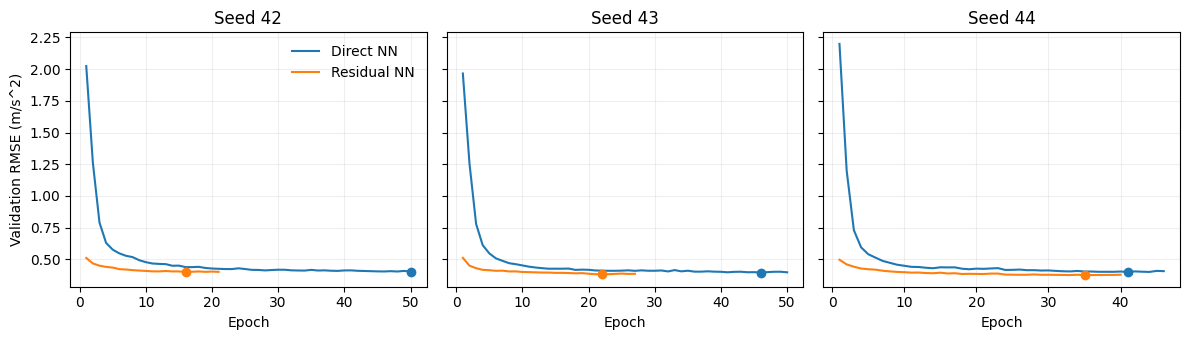
\includegraphics[width=0.94\linewidth]{figures/learning_curves.png}
\caption{Executed-notebook validation curves for paired seeds. Dots identify restored checkpoints.}
\label{fig:curves}
\end{figure}

The highest-error test flights are \texttt{2021-02-23-17-27-24} and \texttt{2021-02-23-22-54-17}. Their mean residual RMSEs are 1.0653 and 0.8988~\unit, respectively. Figure~\ref{fig:errors} shows each flight's worst segment. The first stays below $5$~m/s and has a startup mismatch: recorded $z$ acceleration is about 9.7~\unit\ while both predictions are much smaller. This suggests an unmodeled operating regime. The second contains faster motion and poorly captured vertical peaks. Residual prediction has higher $z$ RMSE in both selected segments. All rows remain in the principal scores; full three-axis plots accompany the results.
\begin{figure}[h]
\centering
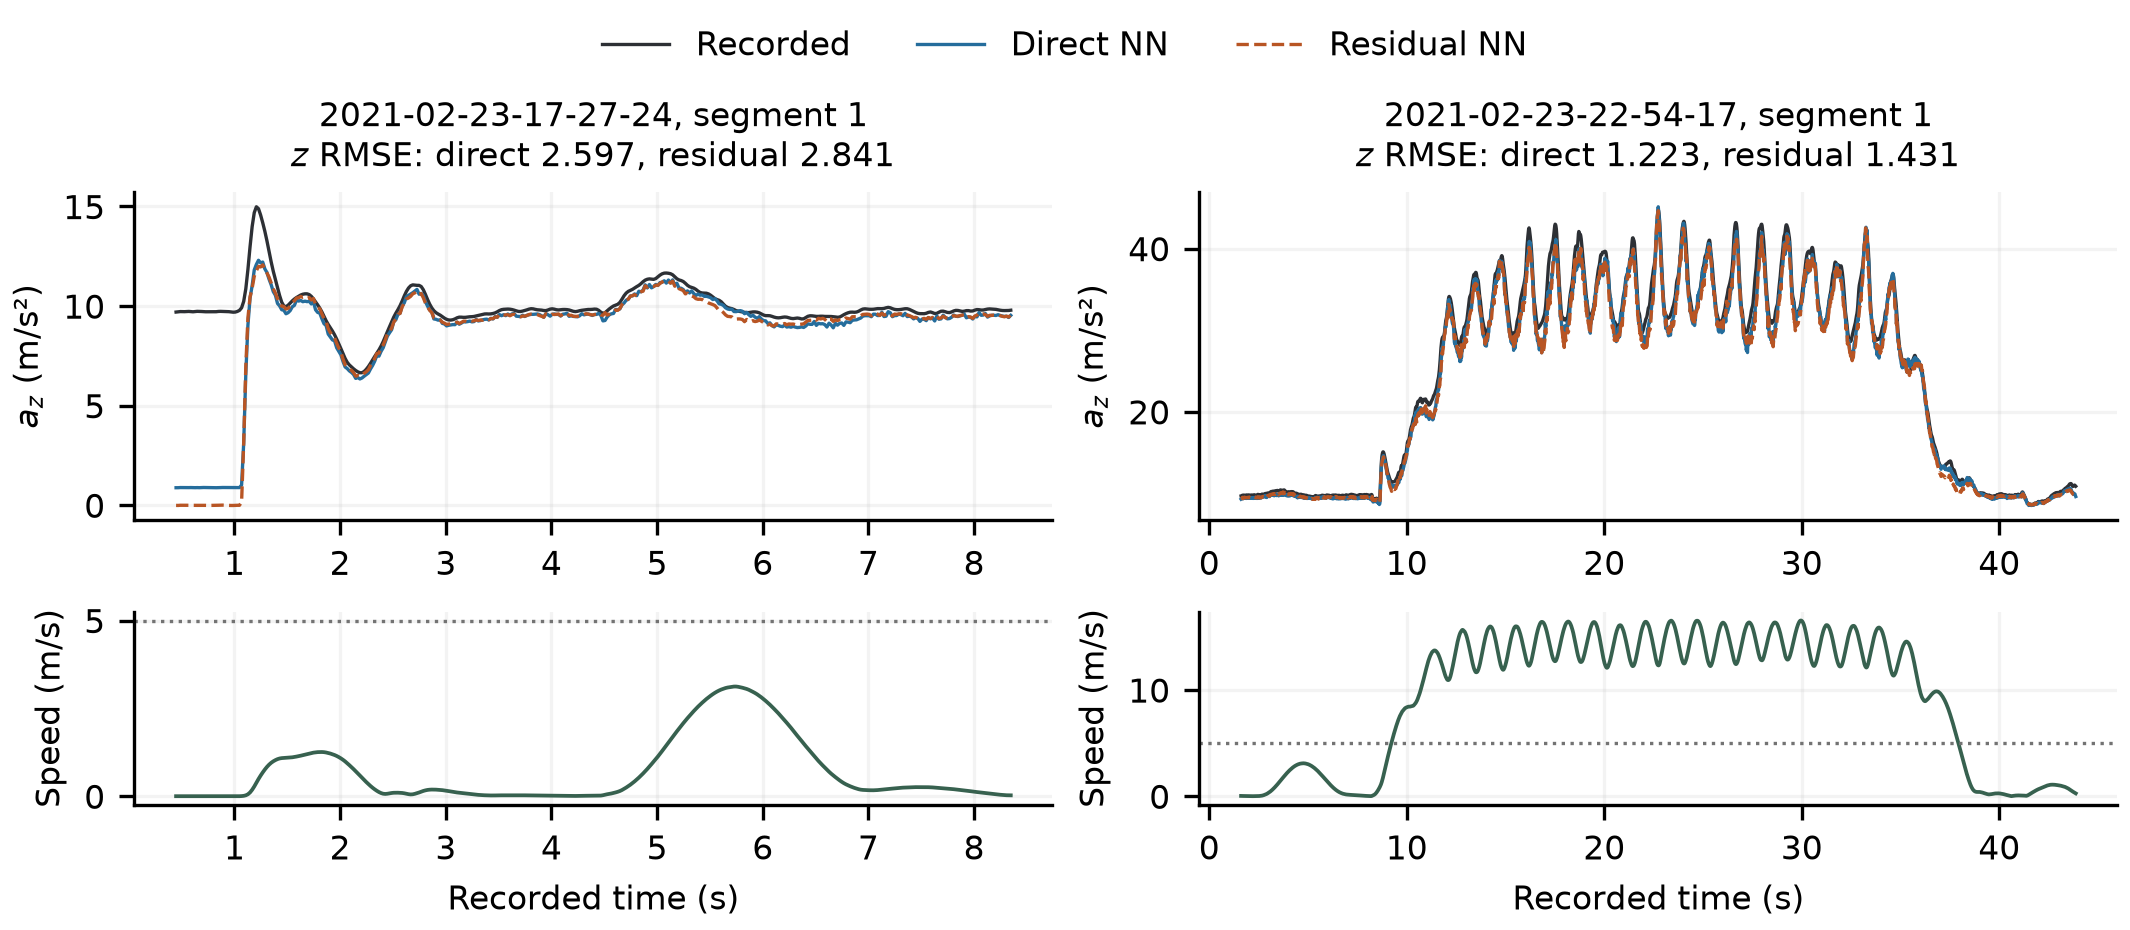
\includegraphics[width=0.94\linewidth]{figures/high_error_compact.png}
\caption{Selected worst segments, seed 42. Actual timestamps and the predefined speed boundary are retained. These post-hoc examples do not estimate failure frequency.}
\label{fig:errors}
\end{figure}

\paragraph{Exploratory comparison across flights.}
For each faster flight, RMSE is scored per seed and averaged. Residual prediction beats direct prediction on 10 of 12 flights and ridge on all 12. Equally weighting flight-level residual-minus-direct differences gives $-0.0260$~\unit. A percentile bootstrap of whole-flight differences (20,000 resamples, seed 42) gives an approximate 95\% interval of $[-0.0430,-0.0083]$~\unit. A two-sided exact sign test gives $p=0.0386$.

This analysis follows test inspection, has no multiplicity correction, and assumes independent flights. Collection sessions may share conditions. Resampling flights avoids treating correlated rows as independent replicates, but does not remove these broader dependence or selection concerns. The interval and $p$-value remain exploratory.

\clearpage
\section{Isaac Sim braking and gust-recovery showcase}
\textbf{NVIDIA Isaac Sim 6.2 simulates the quadrotor motion using PhysX at 120~Hz.} Each 24~s trial starts at 3 or 6~m/s, brakes over three seconds, and holds a 2.3~m waypoint. Lateral winds act at $+2$~m/s during $[1,2)$~s and $-3$~m/s during $[10,12)$~s. All controllers share mass (0.772~kg), inertia, gains, motor mixing, saturation, and 0.04~s rotor lag. The hand-designed drag force is
\begin{equation}
 \mathbf F_d=-m\bigl(0.20\,\mathrm{s^{-1}}+0.04\,\mathrm{m^{-1}}\|\mathbf v-\mathbf w\|_2\bigr)(\mathbf v-\mathbf w),
\end{equation}
where $\mathbf w$ is wind and $\mathbf v$ is world velocity. This plant does not reproduce NeuroBEM aerodynamics.

Learned controllers rotate predicted body $x/y$ acceleration into world horizontal compensation, clip its norm to 3~m/s$^2$, and taper it by $\min(1,\|\mathbf v_{xy}\|_2/(2\,\mathrm{m/s}))$. They do not observe wind or use predicted $z$ acceleration. The thrust controller omits learned compensation. Position RMSE is $\sqrt{N^{-1}\sum_i\|\mathbf p_i-\mathbf p_i^{\mathrm{ref}}\|_2^2}$.

\begin{table}[H]
\centering\small
\caption{Position RMSE in cm, mean $\pm$ sample SD over three model seeds. Tracking uses all 24~s; post-gust uses $t\geq12$~s. Thrust repeats are deterministic.}
\begin{tabular}{@{}lrrr@{}}
\toprule
Controller &Tracking, 3~m/s&Tracking, 6~m/s&Post-gust, 6~m/s\\
\midrule
Thrust &12.341 $\pm$ 0&19.890 $\pm$ 0&10.258 $\pm$ 0\\
Direct &10.608 $\pm$ 0.184&\textbf{10.850 $\pm$ 0.183}&10.305 $\pm$ 0.008\\
Residual &10.639 $\pm$ 0.109&11.099 $\pm$ 0.232&10.260 $\pm$ 0.018\\
\bottomrule
\end{tabular}
\label{tab:sim}
\end{table}
\begin{figure}[H]
\centering
{\small\textbf{(a) Braking gust, simulation time 1.80~s}}\par\vspace{2pt}
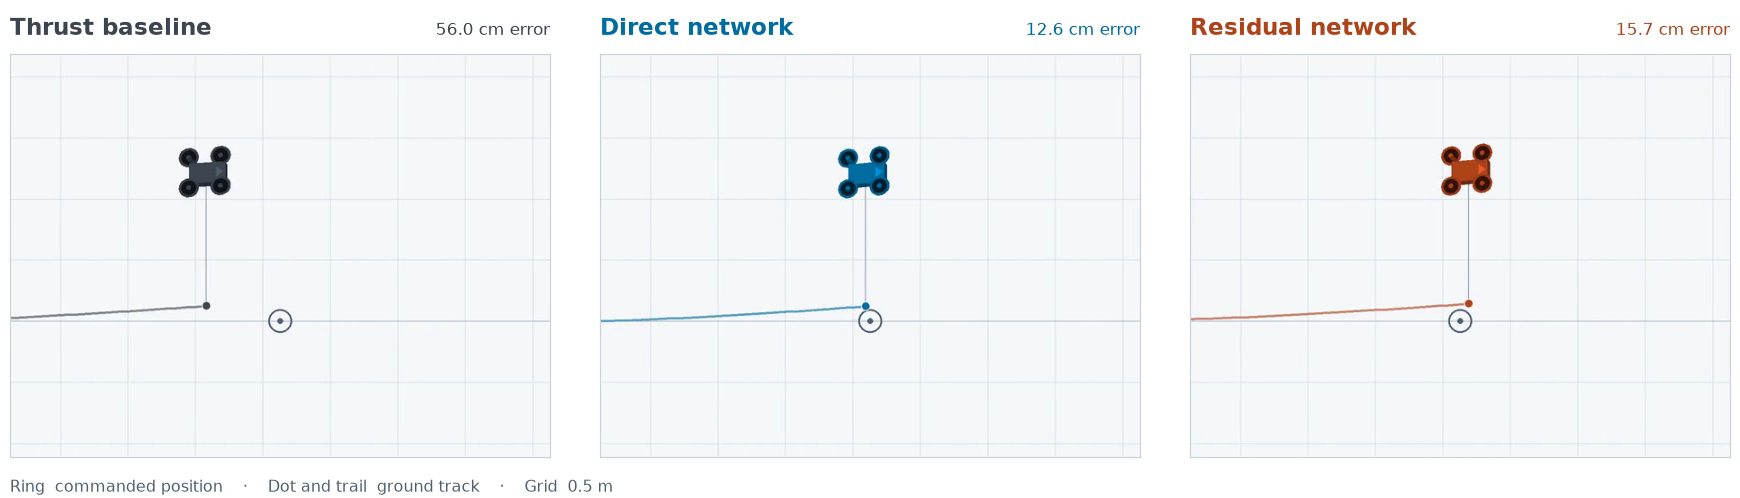
\includegraphics[width=0.96\linewidth]{figures/snapshot_braking_views.png}\par
\vspace{4pt}
{\small\textbf{(b) Hover gust, simulation time 11.80~s}}\par\vspace{2pt}
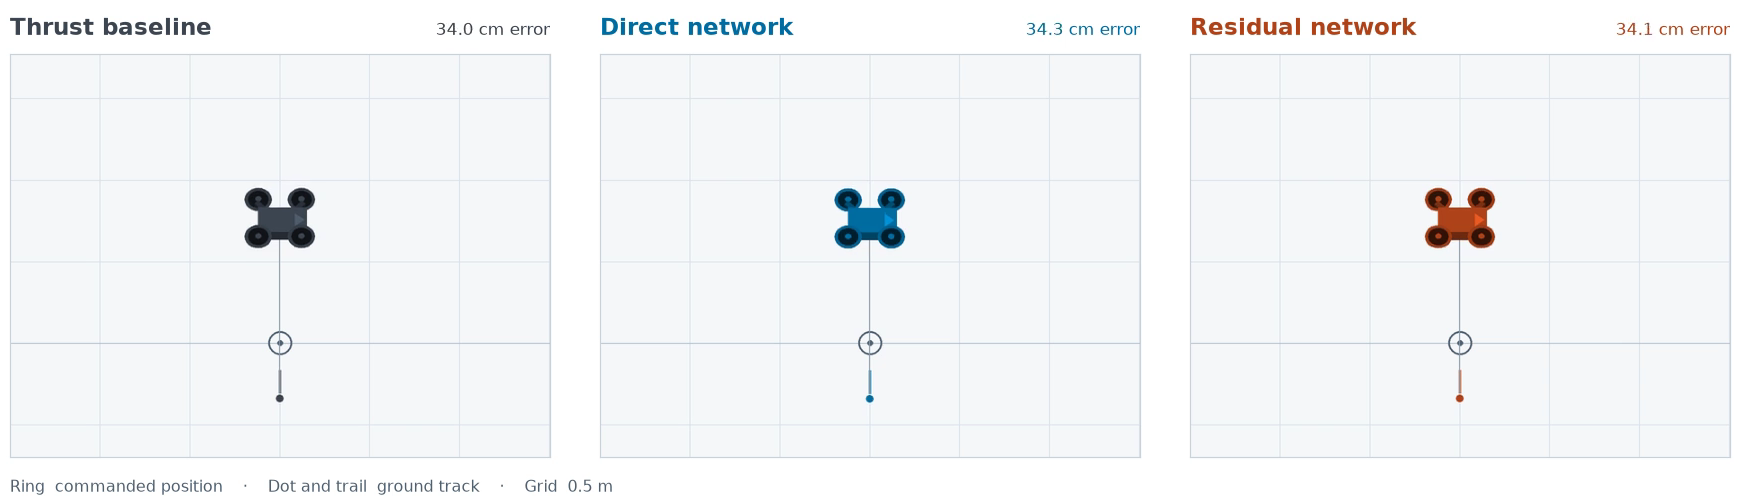
\includegraphics[width=0.96\linewidth]{figures/snapshot_hover_views.png}
\caption{Drone-video snapshots, 6~m/s and seed 42. Isaac Sim/PhysX computes poses; Python renders the views. Rings mark commands; dots/trails show ground tracks. The \href{run:../presentation/media/drone_demo.mp4}{video} replays 24 simulated seconds in 13.2~s, with quiet intervals at $4\times$.}
\label{fig:sim}
\end{figure}

Both learned controllers improve tracking over thrust, but residual RMSE is $2.3\%$ higher than direct. Figure~\ref{fig:sim} shows smaller braking errors and similar hover-gust drift. Post-gust residual/direct RMSE differs by only 0.045~cm. All 18 trials recover without floor violations; direct/residual recovery delays differ by one simulation step.

\clearpage
\section{Interpretation, project evolution, and future work}
The primary hypothesis receives qualified support. The residual model offers a small advantage for the predefined faster group, while direct prediction wins in the slower group. The larger gains arise from moving beyond linear models. Vertical error remains the dominant unresolved channel. A scalar nominal term may simplify some vertical target structure, but the present comparison does not isolate a physical causal explanation. Architecture, target magnitudes, initialization, and stopping behavior can all contribute. The simulation's reversed ranking reinforces that supervised loss alone cannot establish controller quality.

\subsection{Changes from the proposal}
The final implementation retains the proposed ten features, flight grouping, stride-eight sampling, nominal model, linear baselines, matched 32-unit networks, three seeds, and fixed speed threshold. The initial three-file exploration is replaced by an archive-wide audit and the full flight partition. The planned Streamlit viewer becomes an \texttt{ipywidgets} flight selector inside the notebook, reusing the same diagnostic plotting function and avoiding a separate application. The proposal's multi-model selection interface is simplified to simultaneous direct/residual traces with speed. The Isaac Sim braking and gust showcase extends the original prediction study to a controlled feedback example. OLS is fitted on training data in the test-evaluation cell; this cell location does not make it a test-trained model. The paired sign test and flight bootstrap are additional exploratory diagnostics. No supplied instructor feedback introduces further requirements.

\subsection{Limitations and specific next steps}
\textbf{Limited independent coverage.} Thirteen test flights from one platform and indoor collection do not establish generalization to other airframes or outdoor wind. Grouped cross-validation within the training/validation pool should quantify split sensitivity, followed by a newly collected untouched test set covering different sessions and environments. Session-level grouping should replace flight grouping when metadata permits it.

\textbf{Temporal sampling and omitted state.} Stride-eight sampling changes effective rates across files and can alias rapid motion. A training/validation-only comparison of strides 1, 4, and 8, plus timestamp-aware filtering, would test this choice. Battery state and rotor-speed derivatives could address omitted dynamics, but their benefit must be tested as prespecified feature ablations with the same grouped partitions.

\textbf{Small architecture comparison.} Three seeds characterize only limited training variability. A larger paired-seed study, longer matched budgets, learning curves, and capacity-matched ablations of the nominal skip term would help distinguish optimization effects from persistent generalization gains. Further model selection must use validation data, rather than repeated inspection of this test set.

\textbf{Prediction-to-control gap.} The showcase varies trained weights, not independent disturbances or physical plants. Before making deployment claims, vary mass, drag, motor lag, wind profiles, and initial states across paired trials. Compare controllers under a held-out identified plant, then conduct safely supervised hardware experiments. Verify acceleration and gravity conventions before using all three predicted channels in a dynamics integrator.

\subsection{Reproducibility and verification}
The supplied executed notebook contains acquisition, audit, grouping, preprocessing, fitting, scoring, learning curves, and checkpoint export. The accompanying reproduction guide specifies how to rebuild this report and the five-slide deck, rerun the notebook, and regenerate results from the existing checkpoint. The verification script uses the public archive, authors' test list, original flight grouping, and training-fitted scaler to independently recompute the principal tables and paired diagnostics. Saved checksums, numerical outputs, and environment versions accompany it. Simulation metrics are independently recomputed from all 51,858 saved trajectory rows, agreeing with the supplied CSV to numerical precision. This verification reuses trained weights and saved trajectories; it does not claim a fresh neural training run or a new Isaac Sim execution.

\clearpage
\section{Generative AI disclosure and conclusion}
\subsection{Tools, tasks, and verification}
The author reports using \textbf{OpenAI ChatGPT} to help connect to Dartmouth's computing cluster, use Isaac Sim, and reason about introducing residual learning. The original proposal also disclosed AI assistance with topic selection, literature discovery, drafting, and the preliminary notebook. The exact ChatGPT model versions and a complete historical interaction log are not available in the supplied materials, so no such details are inferred.

For this final preparation, \textbf{OpenAI Codex} reviewed the proposal, rubric, executed notebook, trained checkpoint, simulation code, and saved trajectories. Codex drafted and revised the report and Beamer slides, prepared the presentation notes and reproducibility instructions, and wrote the accompanying verification and plotting scripts. AI-assisted material therefore appears throughout the current report and slides, in the added reproducibility files, and in earlier conceptual and cluster/simulation work described above. This disclosure does not attribute the entire pre-existing codebase to a particular AI tool because its authorship history is not fully recorded.

Checks in this preparation include tracing numerical claims to executed outputs, recomputing checkpoint predictions and baseline scores, recomputing simulation metrics from saved trajectories, checking primary reference metadata and dataset documentation, and compiling and visually reviewing the final PDFs. Interpretations were revised to retain the direct model's low-speed advantage, the small residual gain, the exploratory flight-level inference, and the simulation's reversed tracking ranking. These checks were performed with Codex assistance; no independent human verification is claimed here. The author must review the generated material and understand the submitted methods before submission.

\subsection{Conclusion}
A small learned correction substantially improves a weak thrust baseline, but its advantage over a matched direct neural network is modest and depends on speed. Residual learning achieves the lowest faster-group prediction RMSE, while direct prediction performs best below $5$~m/s and tracks slightly better in the 6~m/s simulation. The appropriate conclusion is that the hybrid formulation is promising for acceleration regression under these conditions. Broader claims require more independent flights, matched optimization studies, and stronger control experiments.

\bibliographystyle{unsrt}
\bibliography{references}
\end{document}
